\section{Conceptual description}
\label{sec:concept_descr}

The gathered data of interest originate from the surface of an area corresponding to one mile of the ancient Via Appia in Rome. Conceptually these are divided into road data (also referred as to the {\em background}), which serve as a reference system and context and monument data, which represent the objects of interest, aligned with the road data. The monuments, are referred to as {\em sites}. 

The data, depending on the way of acquisition, are of several types:
\begin{itemize}
\item {\em Point clouds (PC)}
\begin{itemize}
\item A low resolution PC of the research area that has been generated making use of Fugro's DRIVE-MAP services. 
\item High resolution PCs of the different objects of interest (monuments, sites) generated using photogrammetric technologies. 
\end{itemize}
\item {\em Meshes} (sites reconstructions) for different historical epochs. 
\item Contemporary and historical {\em pictures} or paintings. 
\item {\em Attributes} data for the sites and their parts, which are gathered by field observations. 
\end{itemize}

\subsection{Point clouds}
Using the DRIVE-MAP service of Fugro the part of the surface of the Via Appia between the fifth and sixth miles was scanned and a {\em PC} was produced. A point in the PC has 3D coordinates ($x, y, z$), in respect to a given Earth reference system known at scanning time, color and possibly other measured attributes. The resolution (number of points per area or volume) of this point cloud is not enough to see detailed features of the sites, furthermore, they were only scanned from the main road. Thus, the back of the sites is missing. This is illustrated on Fig.\ref{fig:viaAppiaPointCloud}.

\begin{figure}[!ht]
\centering
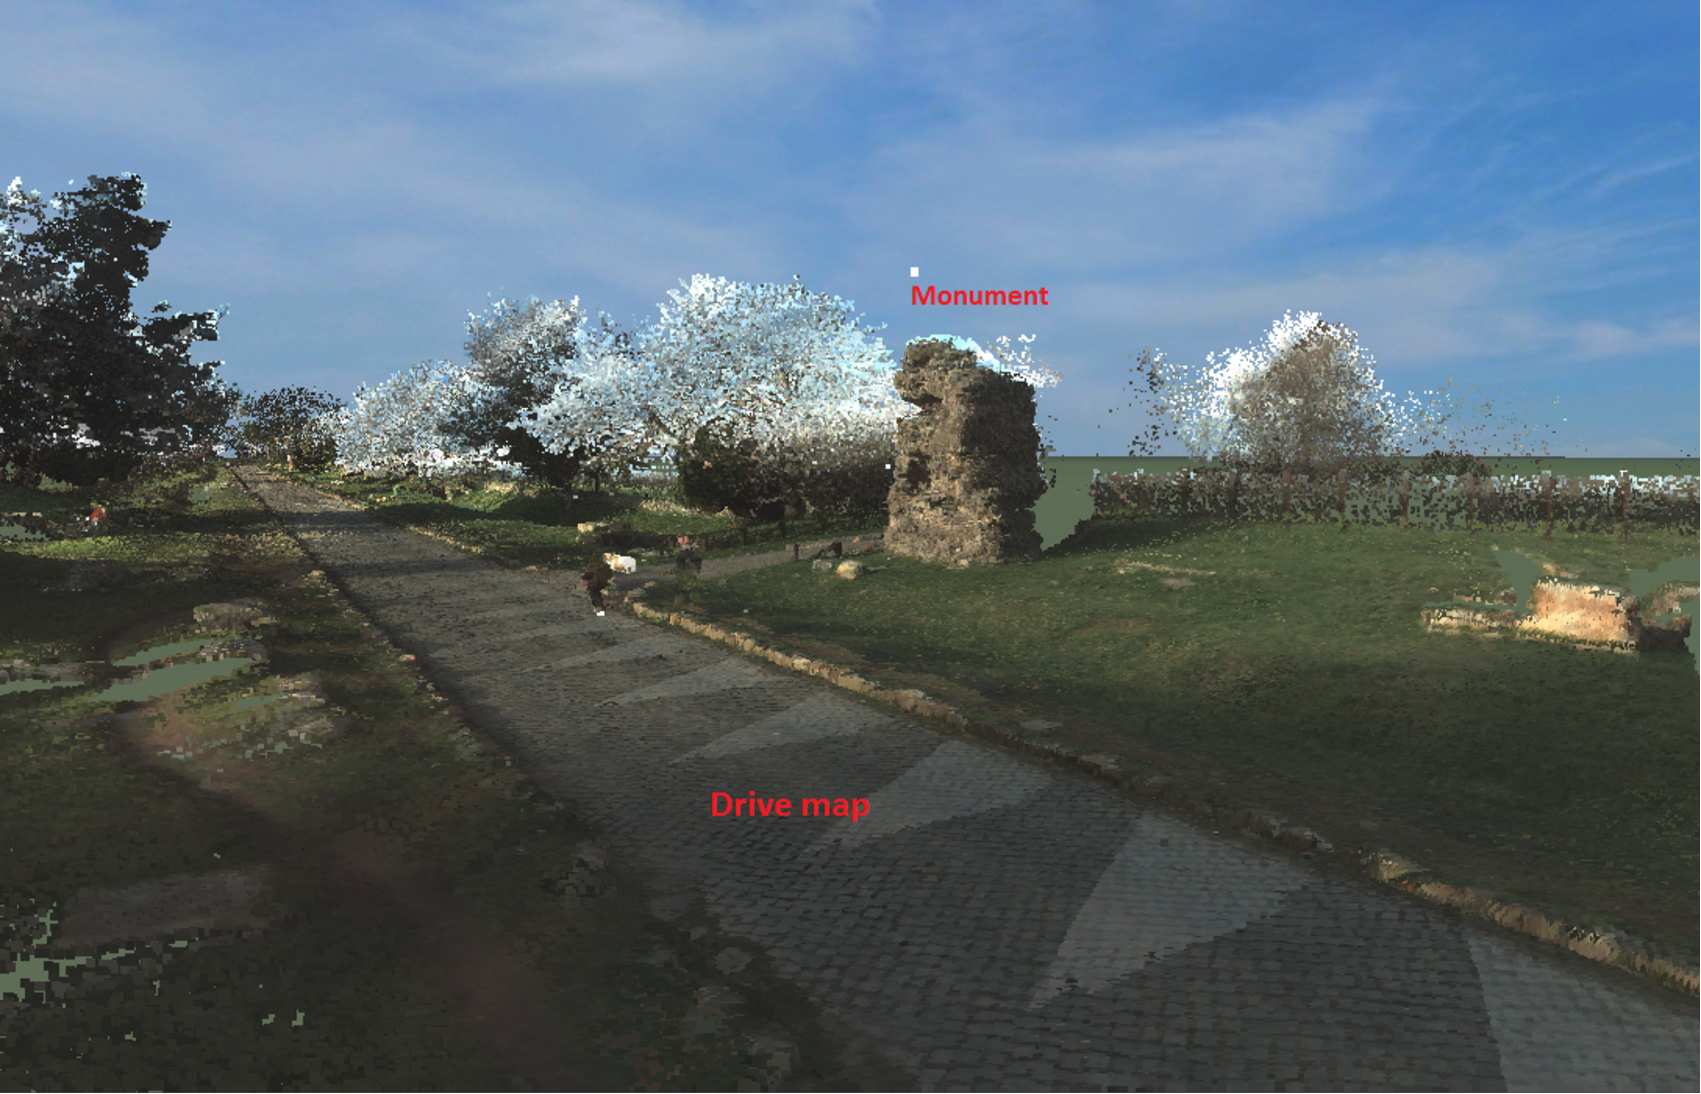
\includegraphics[scale=0.5]{fig/conceptual_description/ViaAppiaPCAnnot.pdf}
\caption{Point cloud data gathered along Via Appia. The Drive map is of low resolution and covers only part of the monuments (sites) facing the road.}
\label{fig:viaAppiaPointCloud}
\end{figure}

Usually there is one drive-map used as a background at a time, while there can be multiple drive-maps obtained at different times or acquisition devices. Or there can be different versions of the same drive-map where some post-processing have been performed like points classification (e.g.\ sky, tree, road, etc.) and possibly non-interesting points filtering (e.g.\ tree and grass removal).

Additional point clouds of higher resolution covering also the back of the monuments have been obtained using photogrammetric software from photographic pictures of the sites from different camera locations (viewpoints). 

\subsection{Pictures}
The pictures of a site can be both contemporary (current) or historical pictures or paintings. An illustration of visualizing a contemporary photo of a monument next to its point cloud data can be seen on Fig.\ref{fig:viaAppiaMeshPicture}. The photo was one of the photos used to generate the high resolution site PC and visualizing it next to the location of the monument can be extra informative or can be used as thumbnail. Usually there are multiple pictures per site.

\subsection{Meshes}
For the purpose of archaeological research, multiple reconstructions of the sites of interest are often performed. These reconstructions, or meshes, can also be current or historical. An illustration of visualizing a contemporary mesh of a monument aligned to its point cloud data can be seen on Fig.\ref{fig:viaAppiaMeshPicture}.

\begin{figure}[!ht]
\centering
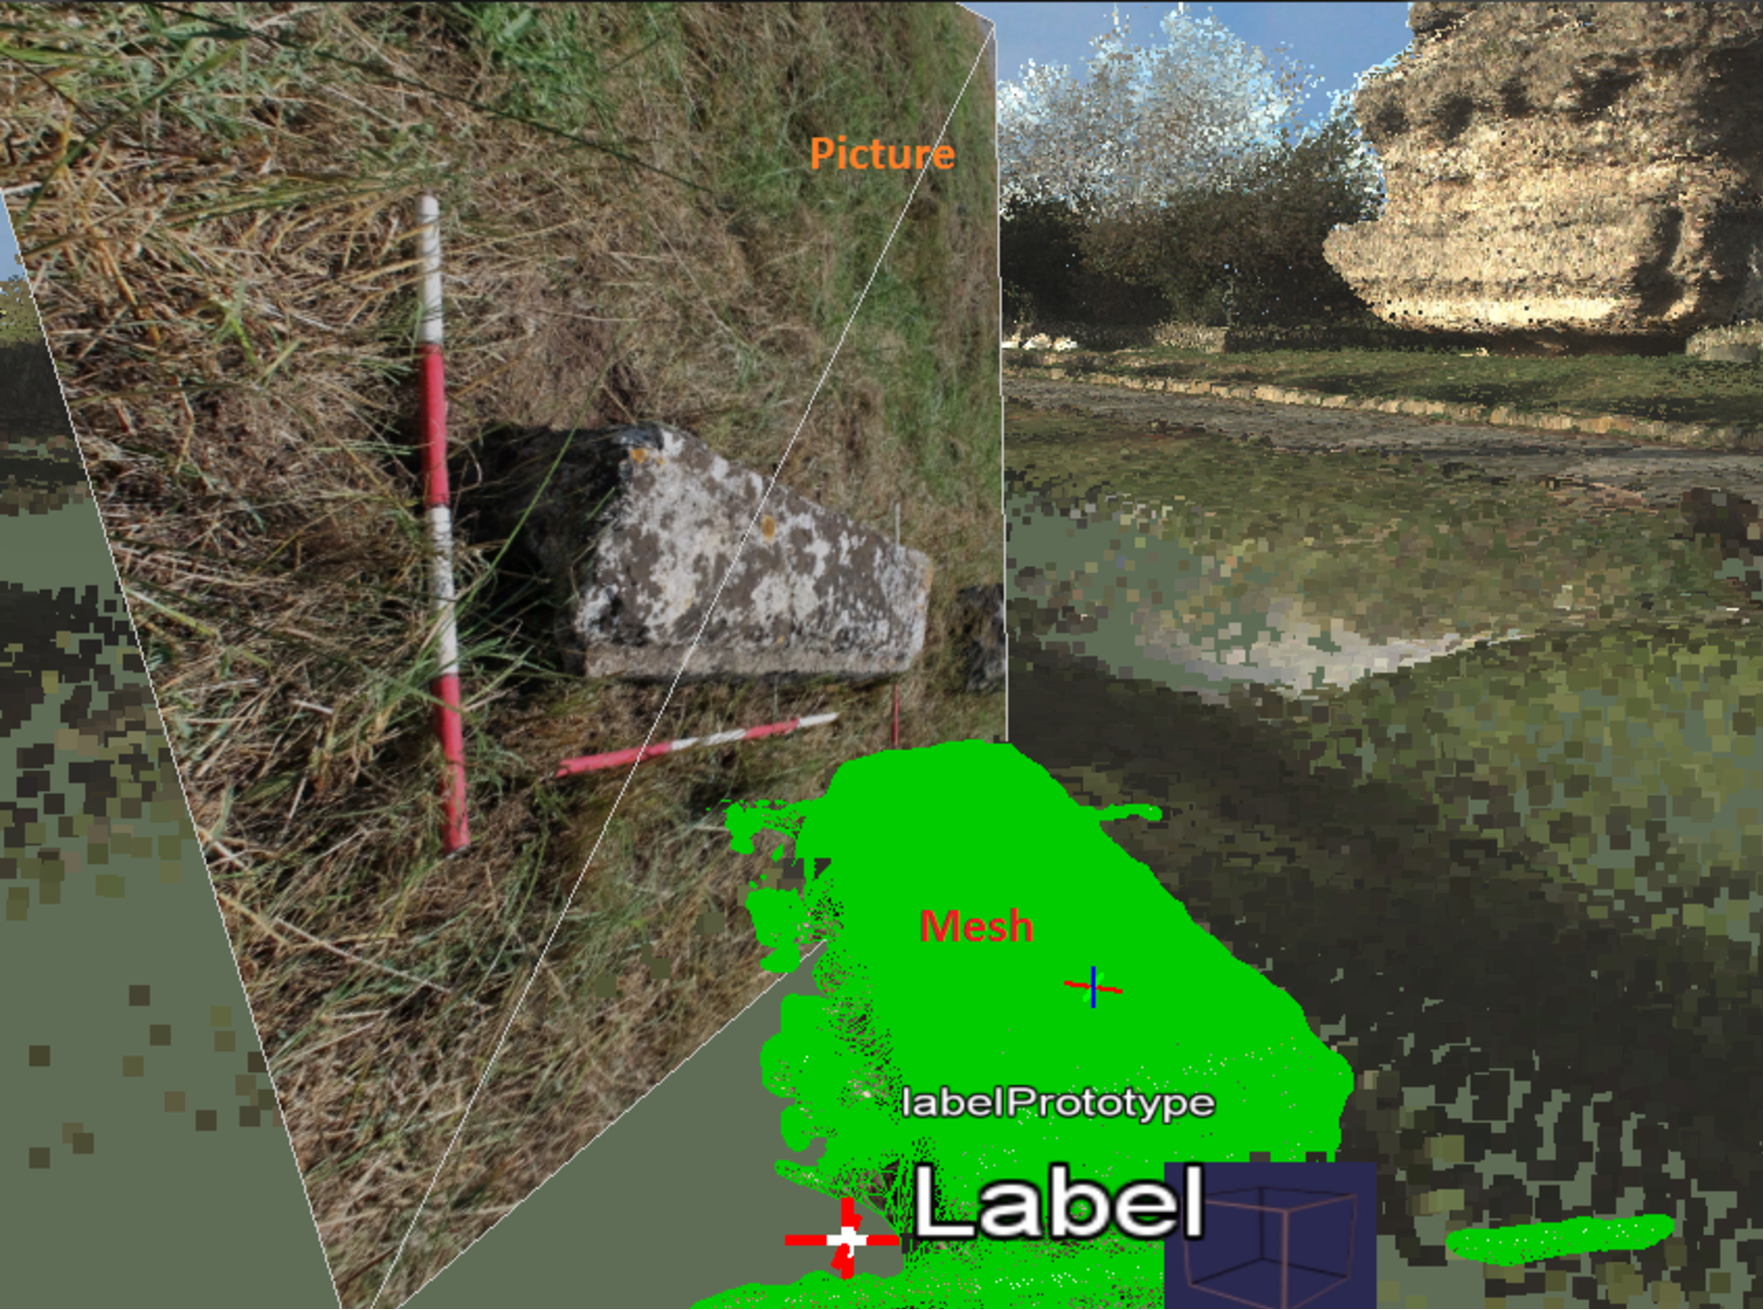
\includegraphics[scale=0.5]{fig/conceptual_description/ViaAppiaMeshPicture.pdf}
\caption{Reconstruction meshes and picture of a site overlayed on the point cloud data.}
\label{fig:viaAppiaMeshPicture}
\end{figure}


The point clouds, meshes and pictures are stored according to the data structure convention (Section \ref{sec:data_structure}).

\subsection {Attributes}
These data are collected on the site from archaeologists. They are relevant to the archaeological research question,  and can be, for example material composition, condition, possible interpretation, description of the different elements or sub-parts, etc.  

The attribute data are considered as additional descriptive (meta) data and are stored in a database along with the pointers to the other data types (Section \ref{sec:database}).